\documentclass[paper=letter, fontsize=11pt]{scrartcl} 
 \usepackage[top=2.5cm, bottom=2.5cm, left=2.5cm, right=2.5cm]{geometry}
\usepackage{framed}

\usepackage{graphicx}
\usepackage{verbatim}
\usepackage{pictex}  
\usepackage{multimedia}
\usepackage{listings}
\usepackage{xcolor,colortbl}
\usepackage[spanish]{babel} % language/hyphenation
\usepackage{amsmath,amsfonts,amsthm} % Math packages
\usepackage{amsbsy}
\usepackage{amssymb}
\usepackage{fancyvrb}
\usepackage{sectsty} % Allows customizing section commands
\usepackage[dvipsnames]{xcolor}

\newcommand{\defi}[3]{\textbf{Definición:#3}}
\newcommand{\fin}{$\blacksquare.$}
\newcommand{\finf}{\blacksquare.}

\newcommand{\grstep}[2][\relax]{%
   \ensuremath{\mathrel{
       {\mathop{\longrightarrow}\limits^{#2\mathstrut}_{
                                     \begin{subarray}{l} #1 \end{subarray}}}}}}
\newcommand{\swap}{\leftrightarrow}

\newcommand{\gen}{\text{gen}}

\newtheorem{thmt}{Teorema:}
\newtheorem{thmd}{Definición:}
\newtheorem{thml}{Lema:}
\newtheorem{thmj}{Ejemplo:}
\newtheorem{thma}{Algoritmo:}

\newcommand{\mub}{\mathbf{\mu}}
\newcommand{\xb}{\mathbf{x}}
\newcommand{\Xb}{\mathbf{X}}
\newcommand{\Simgab}{\mathbf{\Sigma}}
\newcommand{\sumk}{\sum_{k=1}^K}
\newcommand{\sumi}{\sum_{i=1}^n}
\newcommand{\sumj}{\sum_{j=1}^n}
\usepackage{biblatex}
\addbibresource{biblio.bib}

\allsectionsfont{\centering \normalfont\scshape} % Make all sections centered, the default font and small caps
\usepackage{float}
\usepackage{fancyhdr} % Custom headers and footers
\pagestyle{fancyplain} % Makes all pages in the document conform to the custom headers and footers
\fancyhead{} % No page header - if you want one, create it in the same way as the footers below
\fancyfoot[L]{} % Empty left footer
\fancyfoot[C]{} % Empty center footer
\fancyfoot[R]{\thepage} % Page numbering for right footer
\renewcommand{\headrulewidth}{0pt} % Remove header underlines
\renewcommand{\footrulewidth}{0pt} % Remove footer underlines
\setlength{\headheight}{13.6pt} % Customize the height of the header
\usepackage{biblatex}
\addbibresource{references.bib}
\numberwithin{equation}{section} % Number equations within sections (i.e. 1.1, 1.2, 2.1, 2.2 instead of 1, 2, 3, 4)
\numberwithin{figure}{section} % Number figures within sections (i.e. 1.1, 1.2, 2.1, 2.2 instead of 1, 2, 3, 4)
\numberwithin{table}{section} % Number tables within sections (i.e. 1.1, 1.2, 2.1, 2.2 instead of 1, 2, 3, 4)

\setlength\parindent{0pt} % Removes all indentation from paragraphs - comment this line for an assignment with lots of text

\newcommand{\horrule}[1]{\rule{\linewidth}{#1}} % Create horizontal rule command with 1 argument of height

\title{	
\normalfont \normalsize 
\textsc{Centro de Investigaci\'on en Matem\'aticas (CIMAT). Unidad Monterrey} 
\\ [25pt] 
\horrule{0.5pt} \\[0.4cm] % Thin top horizontal rule
\huge Tarea 4 \\ 
\horrule{2pt} \\[0.5cm] % Thick bottom horizontal rule
}


\author{Enrique Santibáñez Cortés} % Your name

\date{\normalsize\today} % Today's date or a custom date

\begin{document}
\lstdefinestyle{customc}{
  belowcaptionskip=1\baselineskip,
  basicstyle=\footnotesize, 
  frame=lrtb,
  breaklines=true,
  %frame=L,
  %xleftmargin=\parindent,
  language=C,
  showstringspaces=false,
  basicstyle=\footnotesize\ttfamily,
  keywordstyle=\bfseries\color{green!40!black},
  commentstyle=\itshape\color{red!40!black},
  identifierstyle=\color{blue},
  stringstyle=\color{purple},
}

\lstset{breakatwhitespace=true,
  basicstyle=\footnotesize, 
  commentstyle=\color{green},
  keywordstyle=\color{blue},
  stringstyle=\color{purple},
  language=C++,
  columns=fullflexible,
  keepspaces=true,
  breaklines=true,
  tabsize=3, 
  showstringspaces=false,
  extendedchars=true}

\lstset{ %
  language=R,    
  basicstyle=\footnotesize, 
  numbers=left,             
  numberstyle=\tiny\color{gray}, 
  stepnumber=1,              
  numbersep=5pt,             
  backgroundcolor=\color{white},
  showspaces=false,             
  showstringspaces=false,       
  showtabs=false,               
  frame=single,                 
  rulecolor=\color{black},      
  tabsize=2,                  
  captionpos=b,               
  breaklines=true,            
  breakatwhitespace=false,    
  title=\lstname,             
  keywordstyle=\color{blue},  
  commentstyle=\color{dkgreen},
  stringstyle=\color{mauve},   
  escapeinside={\%*}{*)},      
  morekeywords={*,...}         
} 

\maketitle

\section{Proyección de la superficie de los continentes de 2D a 3D}\label{ejercicio1}
El conjunto de datos \texttt{data$\_$world.csv} representan puntos aleatorios dentro de los cincos continentes respectivamente (ver Figura \ref{fig:2D_world}).
\begin{figure}[H]
    \centering
    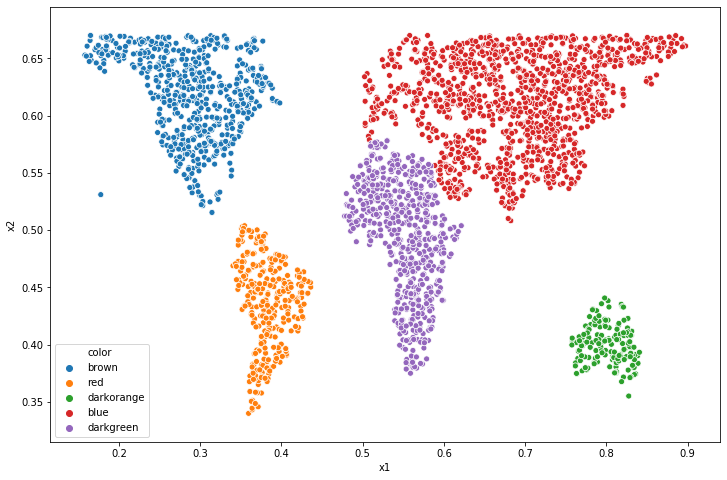
\includegraphics[scale=0.3]{figure/2D_world.png}
    \caption{Data world scatterplot}
    \label{fig:2D_world}
\end{figure}
Ahora considerando el embedding de los datos en una variedad no lineal en 3D (en una esfera,  ver Figura \ref{fig:3D_world3}), es decir, se considera la siguiente parametrización
\begin{align*}
    p = x*(2\pi-0.55), \ \ \ t=y*\pi
\end{align*}
y por lo tanto los datos proyectamos en la variedad no lineal en 3d se representan con las nuevas variables transformadas
\begin{align*}
    x_{esfera} &= \sin(t)*\cos(p)\\
    y_{esfera} &= \sin(t)*\sin(p)\\
    x_{esfera} &= \cos(t)
\end{align*}


\begin{figure}[!htb]
\minipage{0.5\textwidth}
  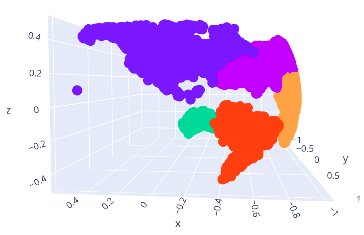
\includegraphics[width=\linewidth]{figure/3D_world1.png}
\endminipage\hfill
\minipage{0.5\textwidth}
  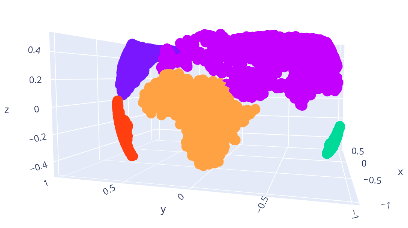
\includegraphics[width=\linewidth]{figure/3D_world2.png}
\endminipage
\end{figure}
\begin{figure}[H]
    \centering
    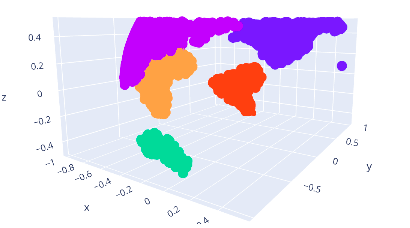
\includegraphics[scale=0.5]{figure/3D_world3.png}
    \caption{Data world proyectados en un esfera, scatterplots 3D}
    \label{fig:3D_world3}
\end{figure}

Entonces el objetivo \textbf{de este trabajo es tratar de reconstruir los patrones encontrados en los datos 2D, a partir de los datos 3D}. Para ello consideraremos los métodos de manifold learning basados en PCA, Kernel PCA, Spectral Embenddings y t$-$SNE. 

\subsection{Ajuste de hiperparámetros}
Considerando los datos 2D, se pueden observar dos tipos de patrones interesantes a buscar: división de los continentes y relación entre los continentes. Es decir, \textbf{en el primero nos interesaría que podemos poder clasificar los puntos en los 5 continentes y el segundo sería como se \textit{relacionan} los continentes entre sí (que tan alejados están los continentes entre sí)}. Es decir, se puede interpretar como la información dentro de los continentes y fuera de los continentes. \\

Procedemos a buscar en cada uno de los métodos de reducción de la dimensionalidad, la mejor combinación de parámetros en donde se pueda observar los patrones anteriores. Para ello el criterio se selección de los parámetros será a \textbf{\textit{ojo}} ya que no tenemos una medida cuantitativa para saber que combinación de parámetros es \textbf{\textit{mejor}}. Se presentan los efectos de cada uno de los parámetros en los distintos métodos, \textbf{para todas las combinaciones se ocupo la semilla igual a "19970808"}. No se presentan todas las combinaciones probadas, solo las más relevantes. 

\subsubsection*{PCA}
Para este método de reducción de dimensión solo consideramos la diferencias del método cuando se aplica al conjuntos de datos sin estandarizar y estandarizado. \\

Observando la Figura \ref{fig:tunning_pca}, notamos que este método no funciona adecuadamente para encontrar los patrones descritos anteriormente. Esto se justifica claramente debido a que el embedding de los datos considera una variedad no lineal y, si recordamos, PCA no sirve para \textit{patrones lineales}. 

\begin{figure}[H]
    \centering
    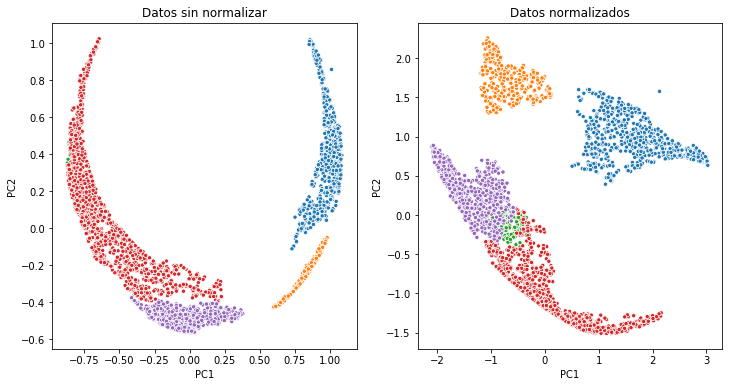
\includegraphics[scale=0.35]{figure/tunning_pca.png}
    \caption{Efecto de la estandarización de los datos.}
    \label{fig:tunning_pca}
\end{figure}

\subsubsection*{Kernel PCA}
En este método existen dos hiperparámetros que afectan la reducción de dimensionalidad: \textbf{\textit{kernel a ocupar} y \textit{coeficiente del kernel}}. Los kerneles que se probaron son \textit{rbf, sigmoid, poly, linear, cosine} (ver \cite{scikit-learn} para mas detalles de las expresiones especificas), y para el coeficiente del kernel probamos los siguientes valores: 0.005, 0.1, 0.2, 0.5, 0.9, 1.4. Este último coeficiente, solo se usa para algunos kerneles (rbf, poly y sigmoid). \\

En total se probaron 17 combinaciones de parámetros distintos, las cuales se probaron en los datos estandarizados y no estandarizados. Primero observemos el efecto que tiene el coeficiente del kernel en un kernel rbf (ver Figura \ref{fig:kpca_gamma}), es fácil ver que entre más grande sea este coeficiente los patrones buscados son difíciles de encontrar. De hecho, para valores mayores a 0.5 se puede observar el problema de crowding. 
\begin{figure}[H]
    \centering
    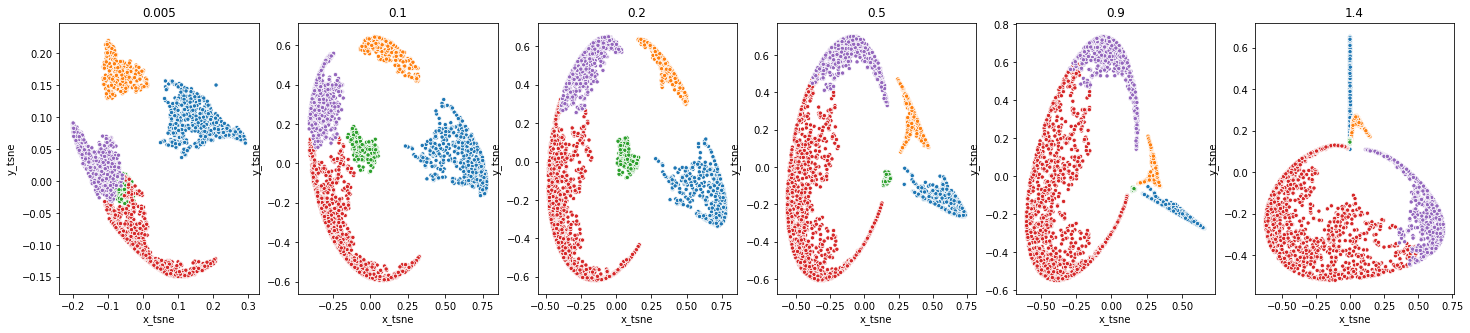
\includegraphics[scale=0.3]{figure/kpca_gamma.png}
    \caption{Efecto de coeficiente del kernel usando kernel rbf.}
    \label{fig:kpca_gamma}
\end{figure}
Ahora, \textbf{veamos que el uso del kernel que ocupemos presenta un mayor impacto en las proyecciones que el coeficiente del kernel} (ver Figura \ref{fig:kpca_kernel}). En las proyecciones de los kerneles \textbf{rbf y cosine} vemos que se puede identificar los puntos en sus respectivos continentes, pero en las proyecciones del kernel rbf no se observa tan claro la relación de los datos entre los continentes. \textbf{Por lo que podemos concluir que la mejor combinación es utilizando el kernel cosine}.  
\begin{figure}[H]
    \centering
    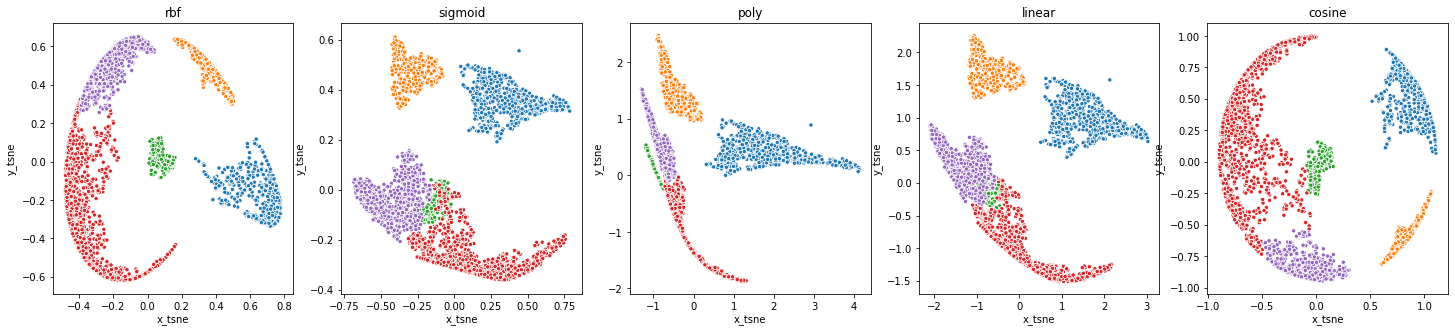
\includegraphics[scale=0.36]{figure/kpca_kernel.png}
    \caption{Efecto de los diferentes kerneles, (coeficiente kernel $=0.2$)}
    \label{fig:kpca_kernel}
\end{figure}
Por último, veamos el efecto que tiene estandarizar los datos antes de ocupar Kernel PCA usando el kernel cosine (ver Figura \ref{fig:kpca_std}). Observemos que cuando no estandarizamos los datos no se observar los patrones originales de los datos en 2D.
\textbf{Por lo tanto, la mejor combinación para este método es usando el kernel cosine en los datos estandarizados} (la proyección de la derecha en la Figura \ref{fig:kpca_std}). 
\begin{figure}[H]
    \centering
    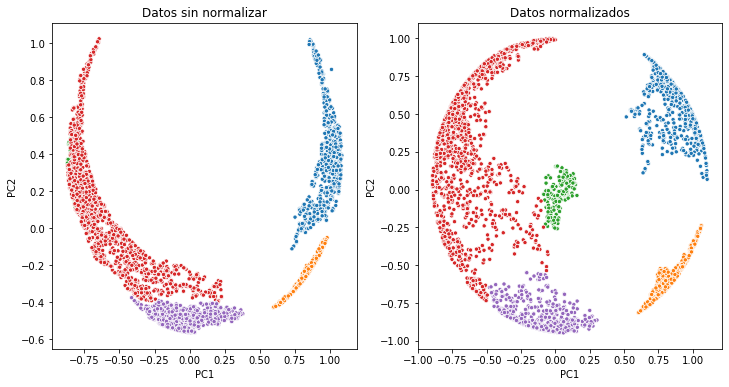
\includegraphics[scale=0.35]{figure/kpca_std.png}
    \caption{Efecto de la estandarización de los datos.}
    \label{fig:kpca_std}
\end{figure}

\subsubsection*{Spectral Embenddings (SE)}
Para este método, los parámetros que afectan el ajuste son: \textbf{construcción de la matriz de afinidad, coeficiente del kernel y número de vecinos más cercanos}. Para la construcción de la matriz de afinidad existen dos maneras de hacerlo: calculando un gráfico de vecinos más cercanos y calculando un núcleo de función de base radial (rbf). Cuando se utiliza vecinos más cercanos se necesita determinar el número de vecinos para el gráfico y cuando se utiliza un núcleo de función de base radial se necesita determinar el coeficiente de kernel. \\

Es decir, probamos SE calculando la matriz de afinidad considerando $(2, 3, 4, 5, 10)$ vecinos más cercanos y calculando la matriz de afinidad usando rbf considerando gamma  $=(.005, .1, .4, .42, .6)$. Se ocuparon los datos normalizados y sin normalizar, pero aquí solo se presentan los datos normalizados. \\

\textbf{El efecto de coeficiente del kernel usando rbf en SE es muy notorio, entre más grande sea (menor a 1) se observan más claros los diferentes cluster} (ver Figura \ref{fig:se_gamma}). Ahora, considerando SE cuando se calcula la matriz usando diferentes números de vecinos más cercanos (ver Figura \ref{fig:se_neighbors}) se observa claramente el efecto, pero este enfoque es erróneo ya que no podemos apreciar ningún patrón. \textbf{Por lo que la mejor combinación para este metodo es considerando rbf y usando el valor de 0.4 como valor del coeficiente de l kernel.}

\begin{figure}[H]
    \centering
    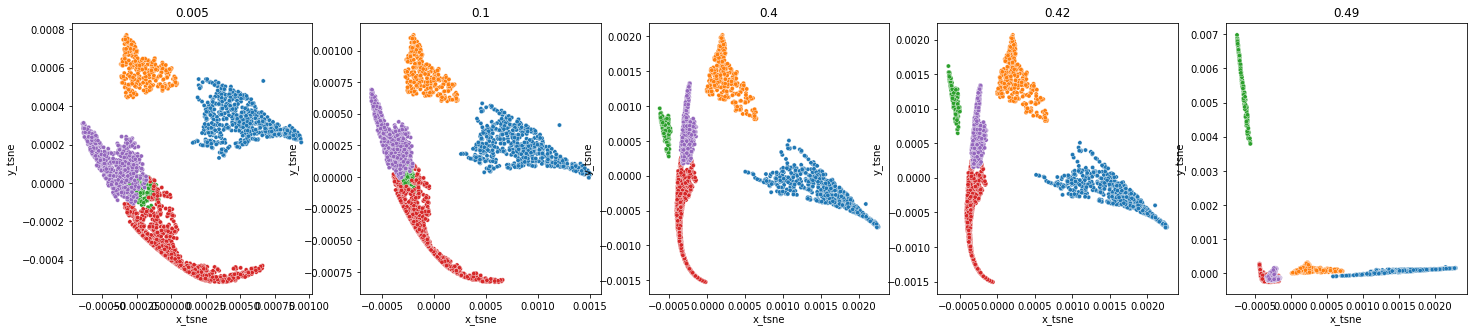
\includegraphics[scale=0.35]{figure/se_gamma.png}
    \caption{Efecto del coeficiente de kernel usando rbf en SE.}
    \label{fig:se_gamma}
\end{figure}

\begin{figure}[H]
    \centering
    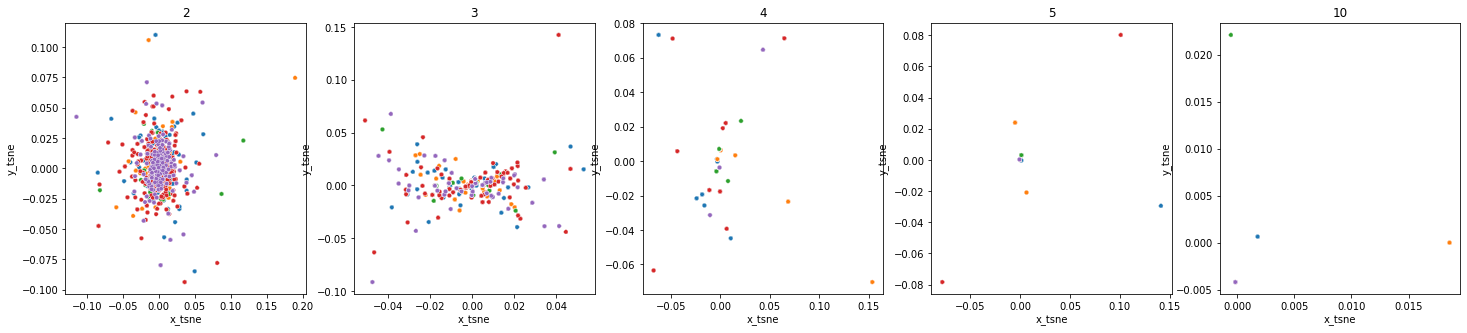
\includegraphics[scale=0.35]{figure/se_neighbors.png}
    \caption{Efecto del número de vecinos más cercanos en SE.}
    \label{fig:se_neighbors}
\end{figure}
\subsubsection*{t$-$SNE}
Y por último, para este método existen diversos parámetros a considerar: \textbf{perplexity, tamaño de aprendizaje y verbose.} Considerar diferentes tamaños de aprendizaje y el verbose distintos no implico diferencias grandes resultados, ya que como tenemos un conjunto de datos pequeño no existen muchas soluciones óptima por lo que cada combinación convergió a la global, por lo cual se omiten los resultados. Entonces se ocuparon los valores de perplexity: $5, 10, 20, 40, 60$. Entre más grande se la perplexity se observan más claro la separación de distintos tipos de grupos, es decir, se hace más claro el patrón de los continentes. \textbf{La mejor combinación sería considerar una perplexity igual a 40.}
\begin{figure}[H]
    \centering
    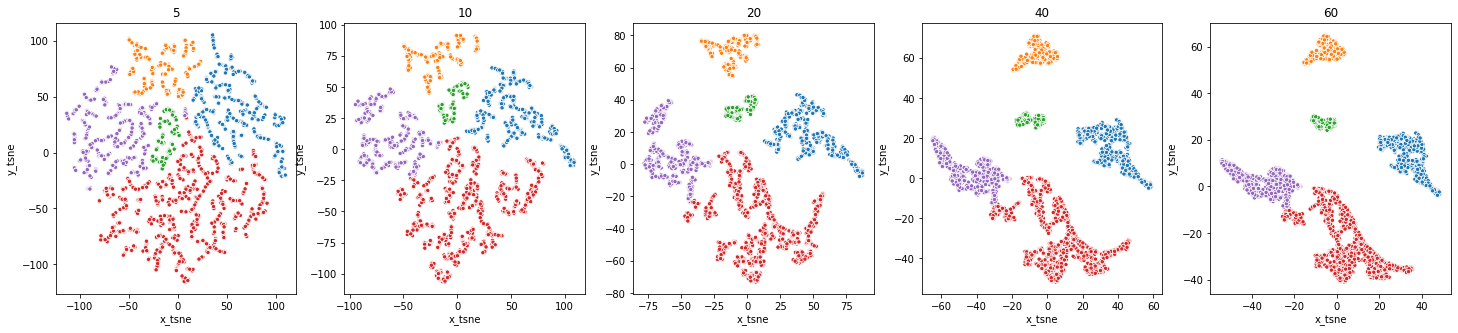
\includegraphics[scale=0.3]{figure/tsne_perplexity.png}
    \caption{Efecto de la perplexity en T$-$SNE}
    \label{fig:tsne_perplexity}
\end{figure}

\subsection{Resumen y Conclusiones}
Por último, compararemos todas las mejores combinaciones de cada método explicado anteriormente (ver Figura \ref{fig:resultados_world}). Recordemos que estamos interesados en tener la información de los continentes dentro y fuera de ellos.\\

\textbf{PCA no logra capturar capturar ninguno de los patrones de los datos originales}, por lo que en este caso es el método con los peores resultados. \\

\textbf{T$-$SNE logra capturar el patrón dentro de los continentes}, es decir, puede separar claramente los puntos por continente. Pero la interpretación fuera de los continentes no es clara, ya que sería un error interpretar la distancia que existen entre estos continentes, por ejemplo, considerar que los puntos naranjas están más alejados de los puntos rojos esto sería un gran error por definición de T$-$SNE.\\

\textbf{En mi parecer los mejores resultados se obtienen cuando se considero Kernel PCA y SE.} Utilizando kernel PCA se puede apreciar los dos patrones del conjunto de datos en 2D, \textbf{solo que desde una perspectiva distinta}. Es decir, en la figura \ref{fig:2D_world} representa un mapa tradicional del mundo y las proyecciones utilizando Kernel PCA representan la proyección del mundo en un plano perpendicular a los polos (proyección polar (ver Figura \ref{fig:proyecciones}), \cite{arggis}).
\begin{figure}[H]
    \centering
    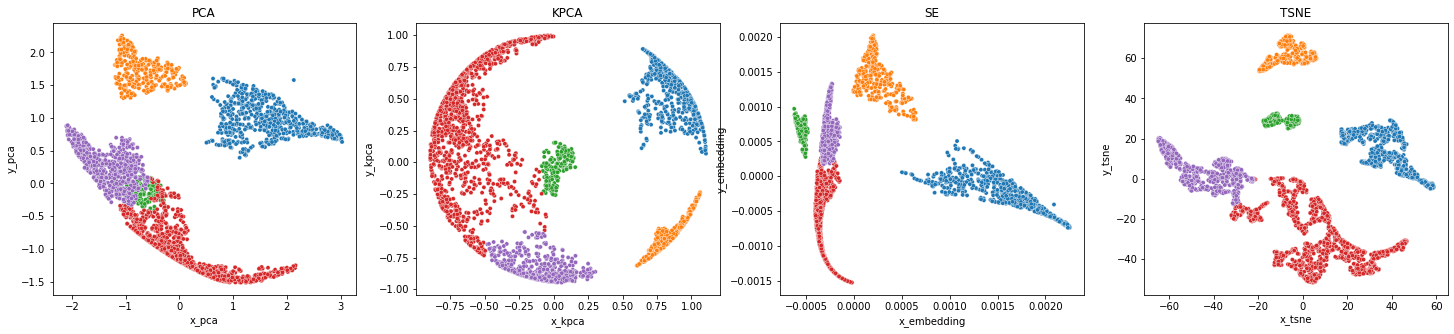
\includegraphics[scale=0.37]{figure/resultados_world.png}
    \caption{Mejores proyecciones de cada métodos.}
    \label{fig:resultados_world}
\end{figure}
En cambio SE, presenta una proyección de los datos que se puede apreciar la información dentro y fuera de cada continente. Es decir, \textbf{podemos decir que esta proyección es más apegada a la original de los datos en 2D.} 
\begin{figure}[H]
    \centering
    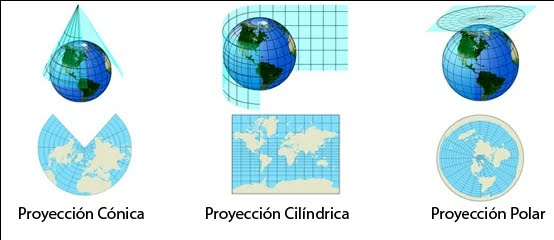
\includegraphics[scale=0.5]{figure/proyecciones.jpg}
    \caption{Proyecciónes geograficas.}
    \label{fig:proyecciones}
\end{figure}

\section{Extensión del problema de los Eigenfaces}
En este ejercicio nos enfocamos al conjunto de datos Labelled Faces in the Wild, que consiste en fotografías de rostros recolectados de internet y contenido en \texttt{sklearn}. Solo se consideraron aquellas personas que tienen al menos 70 fotografías de su rostro en su tamaño original de la imagen $(125\times 94)$.\\

El número total de imágenes analizadas fueron 1288 (ver Cuadro \ref{tab:conteo_imagenes}).

\begin{table}[H]
    \centering
    \begin{tabular}{c|c}
         Nombre& Número de Fotografia \\ \hline \hline
         George W Bush  &  530\\
Colin Powell    & 236\\
Tony Blair      & 144\\
Donald Rumsfeld & 121\\
Gerhard Schroeder  & 109\\
Ariel Sharon    &77\\
Hugo Chavez     &71\\ \hline \hline
    \end{tabular}
    \caption{Número de fotografías por personaje en la muestra.}
    \label{tab:conteo_imagenes}
\end{table}

Si ocupamos en el enfoque tradicional de PCA para reducir el número de variables (en este caso, cada pixel), para poder representar cada fotografía de los rostros en 2D (ver Figura \ref{fig:pca_faces}). Se esperaría que la representación en 2D permitiera identificar los grupos de fotografías por cada uno de los 7 personas que están en todas las fotografías, pero usando PCA esto no es posible. \textbf{Por lo que utilizaremos otros métodos de reducción de dimensionalidad para buscar una representación en donde se observe los 7 grupos esperados.}
\begin{figure}[H]
    \centering
    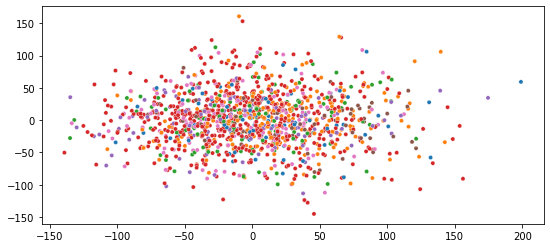
\includegraphics[scale=0.7]{figure/pca_faces.png}
    \caption{Representación de los rostros en 2D.}
    \label{fig:pca_faces}
\end{figure}

\subsection*{Kernel PCA, SE y T$-$SNE.}
Consideramos los métodos de manifold learning basado en Kernel PCA, SE y $t-$SNE para obtener las representaciones en 2D de los rostros. De el Sección \ref{ejercicio1}, nos dimos cuenta de la importancia que tienen los hiperparámetros en estos métodos. \\

Para \textbf{Kernel PCA} se comparo el efecto de: \textbf{kernel a ocupar y coeficiente del kernel}. Se compararon las mismas combinaciones que en la sección anterior (un total de 34 combinaciones), \textbf{y la mejor combinación fue considerando un kernel coseno}. \\

Ahora, para \textbf{SE} los hiperpárametros a comparar fueron: \textbf{construcción de la matriz de afinidad, número de vecinos más cercanos y coeficiente del kernel.} De igual manera, se compararon las mismas combinaciones que en la sección anterior, y \textbf{la mejor combinación fue utilizando los vecinos más cercanos para construir la matriz de afinidad con 7 vecinos más cernanos.} \\

Y por último, para \textbf{$t-$SNE} a diferencia de la sección anterior la tasa de aprendizaje tuvo un efecto notorio, por lo que los hiperpárametros que se compararon son: \textbf{perplexity, tasa de aprendizaje y verbose.} Para este método se probaron alrededor de 50 combinaciones de parámetros, y \textbf{la mejor combinación fue considerando un valor de 40 de perplexity, usando un valor de 15 en la tasa de aprendizaje y verbose igual a 1.}\\

Para no hacer más extenso este trabajo omitimos los efectos que tienen cada uno de los hiperpárametros ya que en la sección \ref{ejercicio1} ya se mostró la importancia de estos, pero para más detalle puede consultar las visualización del archivo \texttt{eigenfaces$\_$plus.ipynb}. 

\subsection{Comparación de los métodos}
Considerando las mejores combinaciones descriptas en la subsección anterior, procedemos a proyectar los datos de las imágenes de los rostros a dos dimensiones (ver Figura \ref{fig:resultados_faces}). \textbf{Cabe resaltar que con ninguno de los cuatros métodos pudo representar los datos de tal manera que se puedan dividir el espacio en el número de personajes que aparecen en las fotografías}, es decir, no es posible representar la información obtenida de todos los pixeles de las fotografías en solo dos dimensiones. Pero si existe una mejoría contra las proyecciones usando PCA.\\

Si comparamos las proyecciones usando PCA (Figura \ref{fig:pca_faces}) con las proyecciones usando Kernel PCA y SE podemos concluir que \textbf{ningún de estos métodos presenta mejorías para poder clasificar los datos por cada uno de los personajes}, parece que los datos están de forma aleatoria en todo el espacio. 
\begin{figure}[H]
    \centering
    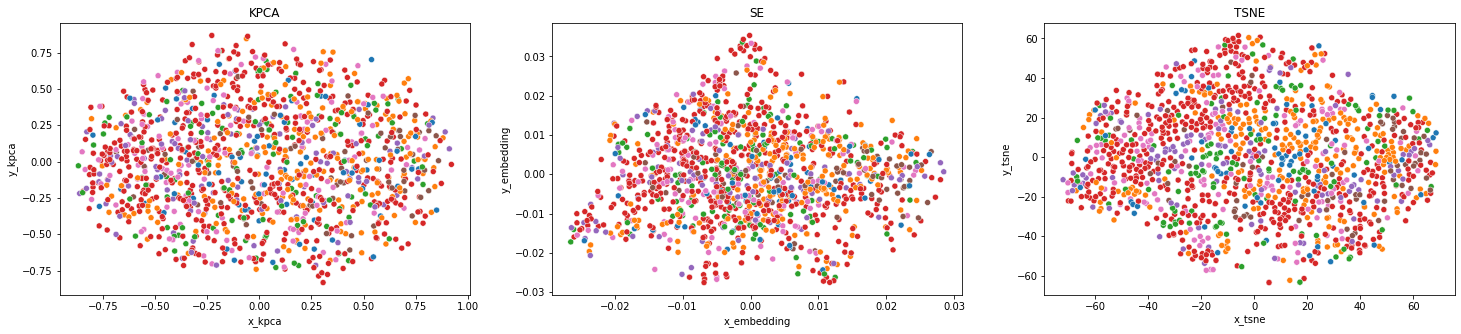
\includegraphics[scale=0.36]{figure/resultados_faces.png}
    \caption{Mejores proyecciones de los rostros en 2D}
    \label{fig:resultados_faces}
\end{figure}
En cambio, si observamos las proyecciones \textbf{usando $t-$SNE se pueden notar pequeñas agrupaciones de fotografías del mismo personaje en todo el espacio} (ver Figura \ref{fig:tsne_final}), es decir, este método no logra separar todas las fotografías de un mismo personajes pero si lograr agrupar algunas fotografías de un mismo personaje, por lo que se considera que este método es mejor que usar PCA, Kernel PCA y SE.
\begin{figure}[H]
    \centering
    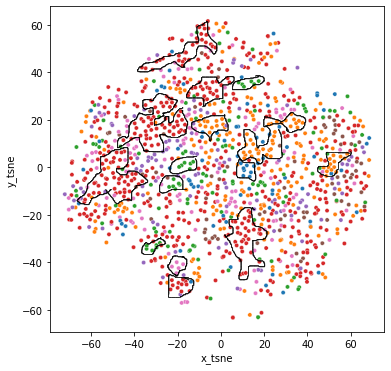
\includegraphics[scale=0.7]{figure/tsne_final.png}
    \caption{Proyecciones de las fotografías usando $t-$SNE.}
    \label{fig:tsne_final}
\end{figure}
Observamos la Figura \ref{hugo} podemos notar que existe una concentración de fotografías de Hugo Chavez en el espacio, pero en esta concentración no están todas las fotografías (los puntos cafes representan las fotografías de Hugo Chavez). 

\begin{figure}[H]
\minipage{0.5\textwidth}
  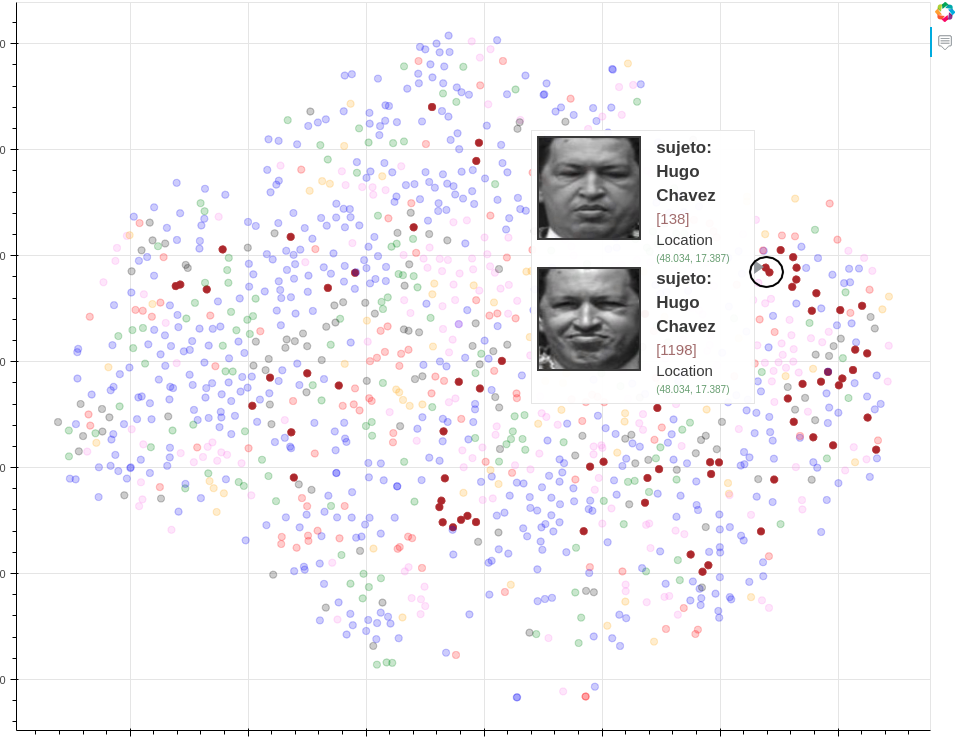
\includegraphics[width=\linewidth]{figure/hugo.png}
  \caption{Fotografías de Hugo Sanchez.}
  \label{hugo}
\endminipage\hfill
\minipage{0.5\textwidth}
  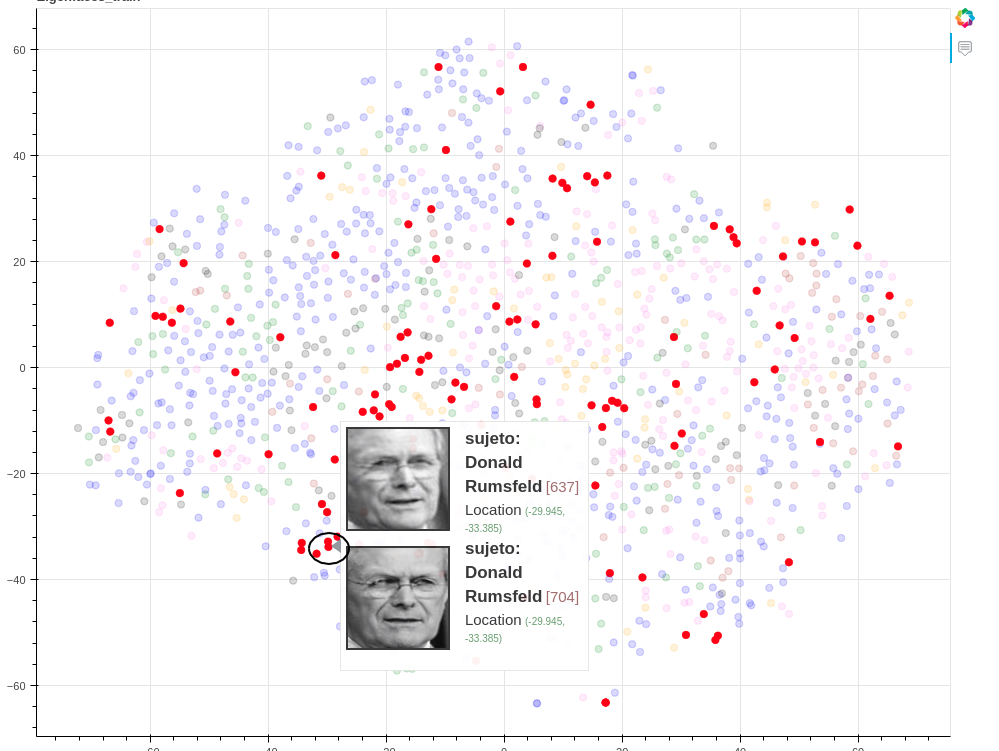
\includegraphics[width=\linewidth]{figure/donald.png}
  \caption{Fotografías de Donald Rumsfeld}
  \label{donald}
\endminipage
\end{figure}

De igual manera, si observamos la Figura \ref{donald} podemos observar algunas concentraciones de las fotografías de Donald Runsfeld (los puntos rojos representan las fotografías de Donald Runsfeld). Además, se puede observar que no existe alguna agrupación que tenga todas las fotografías de Donald Runsfeld, pero si pequeñas agrupaciones con estas.\\

Ahora, intente entender como se forman las agrupaciones (ver Figura \ref{diff}), es decir, \textbf{no solo considerar quien aparece en las fotografías si no si la persona esta sonriendo, con la boca abierta, con lentes, con vista frontal derecha/izquierda, la edad de la persona, etc,} pero como son múltiples combinaciones implica que no sea posible realizarlo de manera manual.
\begin{figure}[H]
\minipage{0.5\textwidth}
  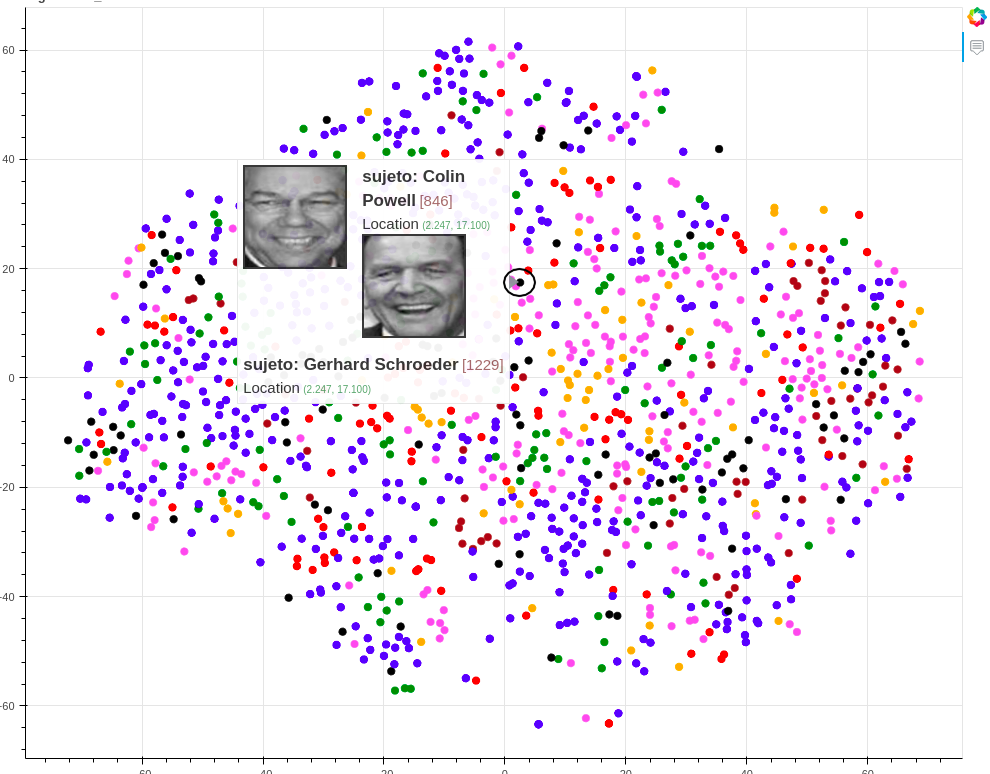
\includegraphics[width=\linewidth]{figure/diff_example.png}
\endminipage\hfill
\minipage{0.5\textwidth}
  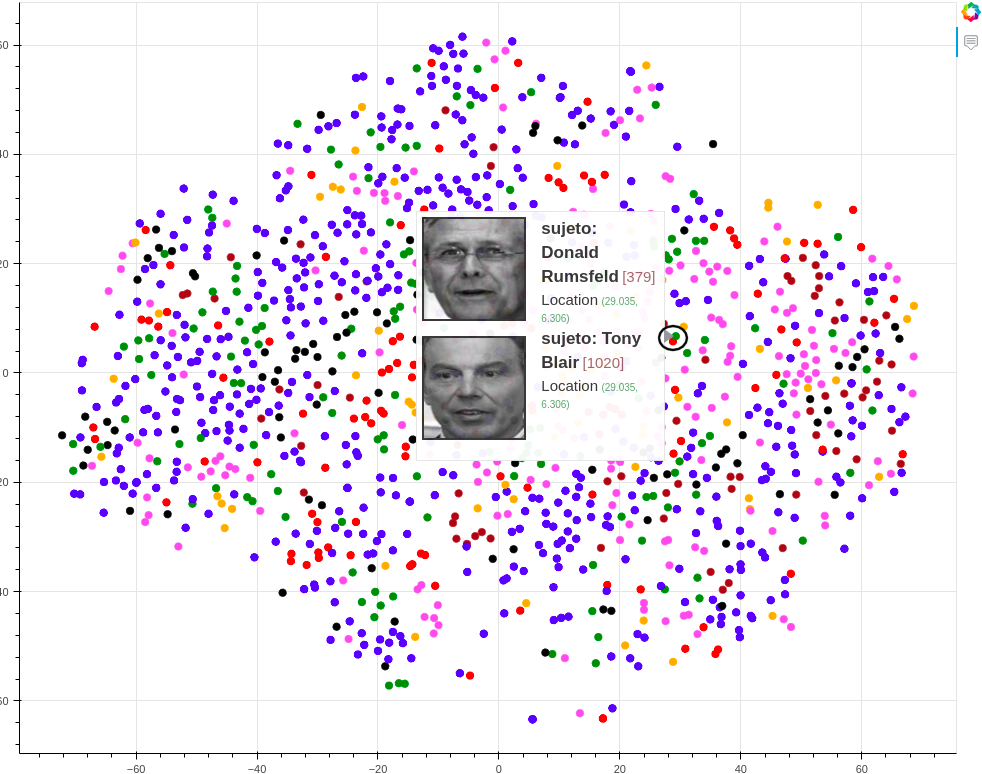
\includegraphics[width=\linewidth]{figure/diff_example2.png}
\endminipage
\caption{Agrupación errónea.}
\label{diff}
\end{figure}

\subsection*{Conclusiones}
En conclusión, \textbf{con ningún método fue posible de proyectar las fotografías de tal manera que se pudieran identificar cada una de los personajes}. La razón por lo cual no se puede es debido a que estamos reducir demasiadas dimensiones para llegar solo a 2, lo que hace que perdamos bastante información. Además, podemos decir que existe una mejor versión de las  proyecciones de las fotografías en 2D, en comparación con las proyecciones de PCA.\\

Recordando un ejemplo muy parecido visto en clase, de las proyecciones de las fotografías de los dígitos usando PCA y cuando se usa $t-$SNE. En este ejemplo vimos que si se puede identificar la mayoría de los 10 dígitos en el espacio por separado, pero en comparación con el ejercicio analizado en este trabajo las fotografías de los dígitos presentan menor información (varianza en sus variables) que las fotografías de los rostros. Por lo que, esta diferencia de información hace posible o no identificar más fácilmente grupos de fotografías en una dimensión más pequeña. 

\subsection*{Anexo}
Todos los códigos utilizados para estos resultados se pueden encontrar en mi página personal de Gitgub: Enriquesec. En el repositorio Ciencia de Datos/Tareas/Tareas$_$4/. El notebook \texttt{world$\_$2d.ipynb} contiene los resultados de la primera sección, y el notebook \texttt{eigenfaces$\_$plus.ipyng} contiene la segunda sección de este trabajo.

\printbibliography



\end{document}